% @file   thesis.tex
% @brief  graduation thesis of Shibaura Institute of Technology
% @author Kataoka Nagi al18036[at]shibaura-it.ac.jp
% @date   2021-12-21 15:19:48
% $Version:   1.0
% @parHistory
% add
% Copyright (c) 2021 Kataoka Nagi

\documentclass[12pt,a4j]{jreport}
\setcounter{secnumdepth}{5}
\usepackage[dvipdfmx]{graphicx}
\usepackage{amsmath,amssymb}
\usepackage{comment}
\usepackage{graphicx}
\usepackage{here}
\usepackage{bm}
\usepackage{url}

\renewcommand{\baselinestretch}{1.5}

\renewcommand{\bibname}{参考文献}





\begin{document}


%%%%%%%%%%%%%%%%%%%%%%%%%%%%%%%%%%%%%
% 表紙
%%%%%%%%%%%%%%%%%%%%%%%%%%%%%%%%%%%%%
\begin{titlepage}

\begin{center}

\vspace*{2cm}
\Large 2021 年度 芝浦工業大学 工学部 情報工学科\\

\vspace*{1.0cm}
\Huge 卒 \qquad 業 \qquad 論 \qquad 文\\
\vspace*{2.5cm}

\Large 記事トピックのクラスタを用いた\\多言語ニュース推薦手法の提案

\vspace{4cm}
\begin{tabular}{ll}
\vspace*{2mm}
学籍番号 & \qquad $\mathbf{AL18036}$ \\
\vspace*{2mm}
氏\phantom{  }名 & \qquad 片岡 \quad 凪   \\
\vspace*{2mm}
指導教員   & \qquad 木村 \quad 昌臣
\end{tabular}
\end{center}
\end{titlepage}



% \begin{abstract}
% このファイルは,情報工学科卒業論文の推奨テンプレートである.概要書とは異なり,卒業論文本体のテンプレートはあくまで推奨であるので,このテンプレートを下にして文字サイズや行間などを修正したものを利用しても良く,またこのテンプレートを使わなくても良い.

% この部分の研究概要では,研究背景,解決したい問題,研究目的,提案手法,評価方法,評価の結果について簡潔に書く.
% 概要の有無は任意.
% \end{abstract}


{\makeatletter
\let\ps@jpl@in\ps@empty
\makeatother
\pagestyle{empty}
\tableofcontents
\clearpage}

\setcounter{page}{1} 
\pagestyle{plain}

%%%%%%%%%%%%%%%%%%%%%%%%%%%%%%%%%%%%%%%%%%%%%%%%%%%%%%%%%%%%
% 書式 
%%%%%%%%%%%%%%%%%%%%%%%%%%%%%%%%%%%%%%%%%%%%%%%%%%%%%%%%%%%%
% 図の参照『図\ref{fig_nn}に3層のニューラルネットワークを示す』
% \begin{figure}[ht]
% 	\centering
% 	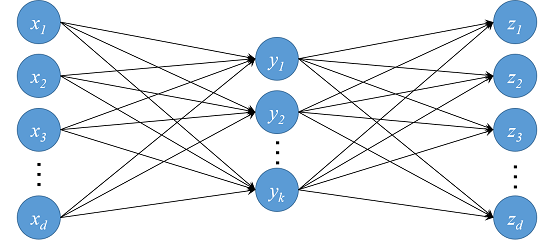
\includegraphics[keepaspectratio, width=120mm]{img/sample.png}
% 	\caption{提案法に用いた3層のニューラルネットワーク.キャプションにはこの図の説明を書く.}
% 	\label{fig_nn}
% \end{figure}

% 表の参照『表\ref{table_a}に手法Aおよび手法Bの正答率を示す』
% \begin{table}[ht]
%   \caption{手法Aおよび手法Bの正解率と平均計算時間.}
%   \label{table_a}
%   \centering
%   \begin{tabular}{lcr}
% \hline
% 手法   & 正解率[\%]  &  計算時間[ms]  \\
% \hline \hline
% 手法A  & 92.3  & 512 \\
% 手法B  & 87.4  & 32  \\
% \hline
%   \end{tabular}
% \end{table}

% 参考文献『井尻らは,X線CTとデジタルカメラを用いた3次元モデリング法を提案した\cite{Ijiri18}.』
% 参考文献リスト『著者1, 著者2,...,著者N. タイトル. 論文誌or学会名, 巻, 号, ページ, 発表年. 』
% Webページ『著者. ページタイトル. ページURL(2021年7月31日参照).』


%%%%%%%%%%%%%%%%%%%%%%%%%%%%%%%%%%%%%%%%%%%%%%%%%%%%%%%%%%%%
\chapter{序論}
%%%%%%%%%%%%%%%%%%%%%%%%%%%%%%%%%%%%%%%%%%%%%%%%%%%%%%%%%%%%

(用紙や文字のなどのサイズには井尻先生のTeXテンプレートをそのまま利用しています)

%%%%%%%%%%%%%%%%%%%%%%%%%%%%%%
\section{研究背景}
~
% @see 

%%%%%%%%%%%%%%%%%%%%%%%%%%%%%%
\section{研究目的}
~
% @see 

%%%%%%%%%%%%%%%%%%%%%%%%%%%%%%
\section{本論文の構成}
~
% @see 

%%%%%%%%%%%%%%%%%%%%%%%%%%%%%%%%%%%%%%%%%%%%%%%%%%%%%%%%%%%%
\chapter{本研究で用いる知識と技術}
%%%%%%%%%%%%%%%%%%%%%%%%%%%%%%%%%%%%%%%%%%%%%%%%%%%%%%%%%%%%

%%%%%%%%%%%%%%%%%%%%%%%%%%%%%%
\section{ニュース推薦システム}
多くのWebニュースサイトでは,様々なアルゴリズムを用いて読者の趣向に合わせた記事が提示されている.
アルゴリズムの例として,
読者が閲覧した記事に似た記事を推薦するコンテンツベースフィルタリング(Content-Based Filtering)や
似た趣向を持つ他の読者の閲覧記事を推薦する協調フィルタリング(Collaborative Filtering),
この2つや他のルールを併用したハイブリッドな手法などがある\cite{karimi_news_2018}.
このような読者にパーソナライズした推薦アルゴリズムをニュース推薦システム(News Recommender Systems)という.
アルゴリズムの評価指標には,記事の閲覧回数,閲覧記事のカテゴリ,読者の位置情報,他サイトの閲覧履歴や購買情報などがある.
% @see News recommender systems – Survey and roads ahead

%%%%%%%%%%%%%%%%%%%%%%%%%%%%%%
\section{ニュース推薦システムが生むバイアス}
パーソナライズするニュース推薦システムは,読者が得る情報に偏りを生む.ここでは,代表的な問題としてフィルターバブル問題とエコーチェンバー問題について記す.本研究は,両問題の部分的な緩和を目指すものである.
% @see 0517-


\subsection{フィルターバブル問題}
Eli Pariserは2011年に,インターネットコンテンツの推薦アルゴリズムにパーソナライズ機能を組み込むことで生じる諸問題をフィルターバブル問題として提唱した\cite{pariser_beware_nodate}\cite{bruns_filter_2019}.
Pariserは,インターネット上で個人の趣向に合わせた限定されたコンテンツばかりが推薦されている状況を,ユーザーが泡の中に閉じ込められたような状態であると例えた.
例として,Facebookでユーザーが支持する政党ばかりが推薦され,Google検索でユーザーの居住地域と関係が薄い時事問題が推薦されるような状況が問題視されている.
泡の中の偏った情報は,新しいアイディアや異なる視点を生みにくくする.
市民が偏った情報ばかりに触れることで,民主主義が機能しなくなる可能性もある.

この泡の中で多様性のある情報を求めることは難しい.
なぜなら,泡の中の情報は個人のキャリアや行動履歴によって決まるため,個人で推薦アルゴリズムをコントロールできないことが多いからである.
同じ理由で,個人が泡の外の情報を特定できないことも大きな問題である.

% (to 提案手法)フィルターバブル問題を緩和する策として,推薦アルゴリズムの公開,個人が推薦アルゴリズムを管理できるオプションの作成,UIの工夫によるバブルの可視化がある.一方で,個人が推薦アルゴリズムを微調節したところで完全に情報の泡から脱することはできないとの指摘もある.UIでバブル内外を可視化しきるのは不可能 情報が多い 手軽

% @see 
% [1]E. Pariser, Beware online 「filter bubbles」, (1304298000). 参照: 1月 06, 2022. [Online Video]. Available at: https://www.ted.com/talks/eli_pariser_beware_online_filter_bubbles
% - きっかけ
%     - Facebook
%         - リベラル派だが進んで保守派と交流する
%         - ある日保守派の人たちが消えた
%         - どのリンクをクリックしているかFacebookがチェック
% - その他の例
%     - Google
%         - 57個のシグナルをチェック
%             - どんなPCを使っているか
%             - どのブラウザを使っているか
%             - 現在地は何処か
%         - 検索結果を調節
%         - 認識しにくい
%             - 自分の検索結果がどれほど他人のものと違うか分からない 
%         - 友人2人がGoogleで「エジプト」と検索
%             - エジプトのデモ関連記事が全くない
%                 - この頃大きな話題だったのに
%             - 他方はそればかり
%     - Yahoo!ニュース,Huffington Post,Washington Post,New York Times
%         - 様々な形でカスタマイズ
% - インターネットは私たちが見たいものを予測して見せている
%     - それは必ずしも見る必要があるものでない
%     - エリック・シュミット「全く何のカスタマイズもされていないものを 人々が見たり利用したりするのは とても難しくなるでしょう」
% - フィルターやアルゴリズムの結果
%     - フィルターに囲まれた世界
%         - あなた個人独特の情報世界となる
%         - 自分の世界に何が含まれるかは自分がどんな人で何をしているかによって決まる
%         - 何が取り入れられるかは自分次第でないのが問題
%             - Netflixのデータアナリスト「「アイアンマン」はすぐ届くのに 「スーパーマン」は 待ち時間が長い」
%                 - 利用者の計画的な向上心と衝動的な今の欲望が大きく対立
%                     - 「羅生門」を観たことがある人になりたい
%                         - 一方で4回目の 「エース・ベンチュラ」を観たい
%                     - 最良の編集は両面を見せる
%                     - フィルターは利用者が何を最初にクリックしたかを主に参考
%                         - そのようなバランスを崩す
%         - **何が削除されるか自分には見えない**
% - 放送社会の創設神話
%     - 編集者が情報の流れをコントロール
%     - インターネットが現れ編集者を追い払った
%     - 私たちは 繋がり合えるようになった
%         - 実際にはそうなっていない
%         - 人間の門番からアルゴリズムの門番にバトンが渡されている
%         - **アルゴリズムは編集者が持ち合わせていた倫理観念をまだ持っていない**
%             - アルゴリズムが関連性以外の要素も必要
%                 - 私たちが何を見て何を見ないか決めるのなら.
%             - 見たくないものや難しいもの,重要なものなども提示
% - 1915年
%     - 新聞は市民としての義務は考慮しない
%     - 市民が適切な情報を得ていないと民主主義は機能しない
%     - 情報のフィルターを行う新聞は重要
%         - ジャーナリズムの倫理が誕生
%     - ウェブ上で同じ問題に直面
%     - プログラムにこの責任を組み込みたい
%         - アルゴリズムを明白に
%         - 何が入ってくるか
%         - フィルターのルール
%         - 自分で何が削除されて何がされないか決められるように管理できるオプション
%         - 新しいアイデアや人々,異なる視点を提示すべき
%         - ウェブ上で私たちが孤立しないように
% [1]和俊笹原, 「ウェブの功罪」, 情報の科学と技術, vol. 70, no. 6, pp. 309–314, 2020, doi: 10.18919/jkg.70.6_309.
% - パーソナライゼーション
% - 選択の条件を知り得ない
% - ブラックボックスであることも
% - **アルゴリズムで虚偽情報が組み込まれることも**
% [1]亜斗夢園田, 寛人中島と不二夫鳥海, 「人気度に着目したニュース閲覧行動の変容分析」, 人工知能学会全国大会論文集, vol. JSAI2020, p. 1L5GS501-1L5GS501, 2020, doi: 10.11517/pjsai.JSAI2020.0_1L5GS501.
% - 自らが好む情報やそれを支持するコミュニティばかり接触することで,偏った考えがより強化される現象
% [1]敏弘神嶌, 昭太郎赤穂, 英樹麻生と淳佐久間, 「情報中立推薦システム」, 人工知能学会全国大会論文集, vol. JSAI2012, p. 3E1R61-3E1R61, 2012, doi: 10.11517/pjsai.JSAI2012.0_3E1R61.
% - フィルターバブル
%     - 利用者が接する情報の範囲に関する問題
%     - 推薦などの個人化技術により,利用者は,知らないうちに,自身が関心があるとされる限定された話題の情報のみにしか接しないようになっており,まるで『泡』の中に閉じ込めらたような状態
%     - 利用者がより新たな話題に関心をもつ機会が奪われたり,社会の中での情報や認識の共有が困難に
%     - フィルターバブル
%     - 推薦を含めた個人化技術によって
%     - 利用者が接する情報の話題の範囲が狭められたり,偏ったりすることが
%     - 利用者が知らないうちに行われるという問題
% [[1]E. BozdagとJ. van den Hoven, 「Breaking the filter bubble: democracy and design」, Ethics Inf Technol, vol. 17, no. 4, pp. 249–265, 12月 2015, doi: 10.1007/s10676-015-9380-y.](https://link.springer.com/article/10.1007/s10676-015-9380-y?source=post_page-----2afbf9cd8367----------------------)
% -  FB
%   -  情報の質の低下
%   -  多様性の低下
% [1]A. Bruns, 「Filter bubble」, Internet Policy Review, vol. 8, no. 4, 11月 2019, 参照: 5月 29, 2021. [Online]. Available at: https://policyreview.info/concepts/filter-bubble
% - フィルターバブル
%     - Eli Pariserが2011年に提唱した概念
%     - 中立的,多様かと思いきや偏っていく
%     - 明確な定義はない
% - 本稿の定義
%     - フィルターバブル
%         - 参加者のグループが,部外者を排除して,お互いに優先的にコミュニケーションをとることを選択したときに発生する(例:Facebookでのコメント,Twitterでの@mentionsなど
%         - 最適化をコントロールしようとする努力もフィルターバブル
% [1]S. NagulendraとJ. Vassileva, 「Understanding and controlling the filter bubble through interactive visualization: a user study」, Proceedings of the 25th ACM conference on Hypertext and social media, New York, NY, USA, 9月 2014, pp. 107–115. doi: 10.1145/2631775.2631811.
% - FBのメリット
%     - 得る速さ
%     - オーバーロードの少なさ
% - FBのデメリット
%     - 偏りに気付かない
%     - 重要だが好き嫌いのある情報が隠れる
%     - ユーザは面白いものにばかりコメントし,囲まれる
%         - 考えさせられる情報
%         - 新しい情報
%     - 開発者に制御される
% - カテゴリのバブル
%     - カテゴリの一般性は高く
%         - 実用上?
%     - Aさんが閲覧した友人Bさんの投稿の1週間のカテゴリービュー
%         - 表示されたらバブル内
%         - Aさんが興味がない可能性
%         - AさんがBさんに共感していない可能性
%         - 過去のいいねした内容に基づく
% - 人間関係のバブル
%     - 逆に,カテゴリーに反応した友人を表示
% [1]広志古賀, 「フィルターバブルとマス破壊兵器について」, 情報経営, vol. 80, pp. 63–66, 2020, doi: 10.20627/jsimconf.80.0_63.
% - フィルターバブル
%   - インターネットの検索履歴がフィルターとなり,同じような情報ばかり表示される(見たくない情報を遮断する)こと
% - フィルターバブル
%     - 無関心圏を拡大
%     - 貢献と誘因の葛藤を放棄
% [1]雅裕片岡, 智訓橋山と俊一田野, 「フィルターバブルを気づかせるシステムの提案」, 人工知能学会全国大会論文集, vol. JSAI2015, pp. 1H21-1H21, 2015, doi: 10.11517/pjsai.JSAI2015.0_1H21.
% - FB
%     - > 推薦システムの発達により利用者が触れる情報は利用者の好みに合う情報ばかりになり,知らず知らずのうちに利用者の興味外の情報や新しい情報などに触れる機会が失われるようになった状態
%     - 社会的リアリティの共有の困難
%     - イデオロギーの極性化
%     - 創造性の低下
% - 問題例
%     - Facebook feed
%         - あまり見てない保守派が突然アルゴリズムで消された
%     - Google検索
%         - 友人に検索させる
%         - 時事的なのエジプト革命でなく,旅行ばかり
% [1]明子小川, 「分断の時代におけるナラティヴとストーリーテリング教育」, 言語文化教育研究, vol. 16, pp. 45–54, 2018, doi: 10.14960/gbkkg.16.45.
% - フィルターバブル
%     - 似た意見や関心を持った人々との間でのみ交流を続ける


\subsection{エコーチェンバー問題}
SNS上で価値観の似た者同士が交流し,共感し合うことにより,偏った意見や思想が反響室のように増幅されて影響力をもつ問題をエコーチェンバー問題という\cite{bruns_filter_2019}\cite{inc_echo_nodate}\cite{nguyen_echo_2020}.
Conoverらや笹原和俊らは,アメリカの選挙期間中のTwitterユーザーが自身の支持する政党に関するツイートを多くリツイートしており,エコーチェンバー問題が生じていることを確認した\cite{conover_partisan_2012}\cite{__2020-5}.

エコーチェンバーの中では,SNSユーザーは自身と異なる価値観や考え方を持つユーザーと交流する機会を失い,偽の情報を訂正する情報を得にくくなってしまう問題もある\cite{__2020-5}.
近年のニュースは読者でコメントを交わすSNSのような性質を有しており\cite{nagulendra_understanding_2014},エコーチェンバーによる情報の偏りを生むと考えられる.
% (to 提案手法)特定の地域の似た文化と価値観を持つ者同士に向けて記事を提供し,読者にコメントさせる事は,エコーチェンバー問題による情報の偏りを生むと考える.

% [5]亜斗夢園田, 喜史関と不二夫鳥海, **「オンラインメディア記事の読者の行動分析」**, 人工知能学会全国大会論文集, vol. JSAI2019, p. 1I2J504-1I2J504, 2019, doi: 10.11517/pjsai.JSAI2019.0_1I2J504.
% - 異なる意見に対する寛容性の低下
% - マイノリティへの偏見の増大
% - フェイクニュースの無批判な受容

% @see 
% [1]和俊笹原, 「ウェブの功罪」, 情報の科学と技術, vol. 70, no. 6, pp. 309–314, 2020, doi: 10.18919/jkg.70.6_309.
% - 似た価値観や考え方をもつユーザーばかりをフォローし,閉じた情報環境ができること
% - 何度も同じ情報を見聞きし,単純接触効果で信じやすくなる
% - 異なる視線のデマ訂正が見えない
% [1]亜斗夢園田, 寛人中島と不二夫鳥海, 「人気度に着目したニュース閲覧行動の変容分析」, 人工知能学会全国大会論文集, vol. JSAI2020, p. 1L5GS501-1L5GS501, 2020, doi: 10.11517/pjsai.JSAI2020.0_1L5GS501.
% - 過度の推薦によってユーザに偏った情報のみを提供し広い視野が失われる現象
% [1]A. Bruns, 「Filter bubble」, Internet Policy Review, vol. 8, no. 4, 11月 2019, 参照: 5月 29, 2021. [Online]. Available at: https://policyreview.info/concepts/filter-bubble
% - 本稿の定義
% - エコーチェンバー
%         - 参加者のグループが,外部の人間を排除して,優先的にお互いにつながることを選択したときに発生する(例:Facebookで友達になる,Twitterでフォローするなど).
% [1]広志古賀, 「フィルターバブルとマス破壊兵器について」, 情報経営, vol. 80, pp. 63–66, 2020, doi: 10.20627/jsimconf.80.0_63.
% - エコーチェンバー現象
%     - 閉塞空間では,見たい情報しか見えないという状況が生まれる傾向が強い
%     - そのために,特定の信念が増幅または強化され,反対意見を受け容れ難くなる
% [1]明子小川, 「分断の時代におけるナラティヴとストーリーテリング教育」, 言語文化教育研究, vol. 16, pp. 45–54, 2018, doi: 10.14960/gbkkg.16.45.
% - エコーチェンバー
%     - 同じような考えや嗜好の人々の間で意見が反響
% [1]Nguyen, C. T. (2020).   Echo Chambers and Epistemic Bubbles Episteme, 17(2), 141-161.
% - 認識論的バブル
%     - 他者の声が欠落によって除外された情報ネットワーク
%     - 不健全なNW
% - エコーチェンバー
%     - 他者の声が積極的に信頼されなくなった社会的構造
%     - 健全なNWにも存在可能
%     - はるかに脅威
%         - 明白な証拠に対する激しい抵抗を説明できる
% - 選択的暴露
%     - 同じ考えをもつ人から情報を得ようとする行為者の傾向
% - 行為者の情報環境は他の行為者によって改変され得る
%     - フィルター技術
%         - アルゴリズムの秘匿性のため,ユーザーは検索結果が調整される度合いを過小評価
%         - フィルターバブルはフィルター技術に限定

% \subsection{エピステミックバブル}

%%%%%%%%%%%%%%%%%%%%%%%%%%%%%%
\section{機械学習}
機械学習は,コンピュータにデータを学習させるコンピュータープログラミングに関する科学技術である\cite{aurellen20}.
ここでいう「学習」は,コンピュータに与えたタスクについて,その評価指標が向上するようなコンピュータープログラミムを実行することを指す.
機械学習を用いることで,既知のアルゴリズムが無い問題を解決したり,データの予想外な傾向を発見したりすることができる.
また,僅かに異なる複数のデータごとにアルゴリズムを用意せずとも実行できる強みをもつ.
以下では,本研究に関連する機械学習に関する知識について記す.

% @see 

\subsection{ニューラルネットワーク}
ニューラルネットワークは,図\ref{fig_nn}動物の脳細胞からヒントを得た機械学習の基本的なモデルである\cite{aurellen20}.
式(\ref{nn_layer})に示すように,複数の入力から1つ以上の出力を得る関数や,この関数をいくつか合成させた関数で表される.

\begin{figure}[ht]
	\centering
	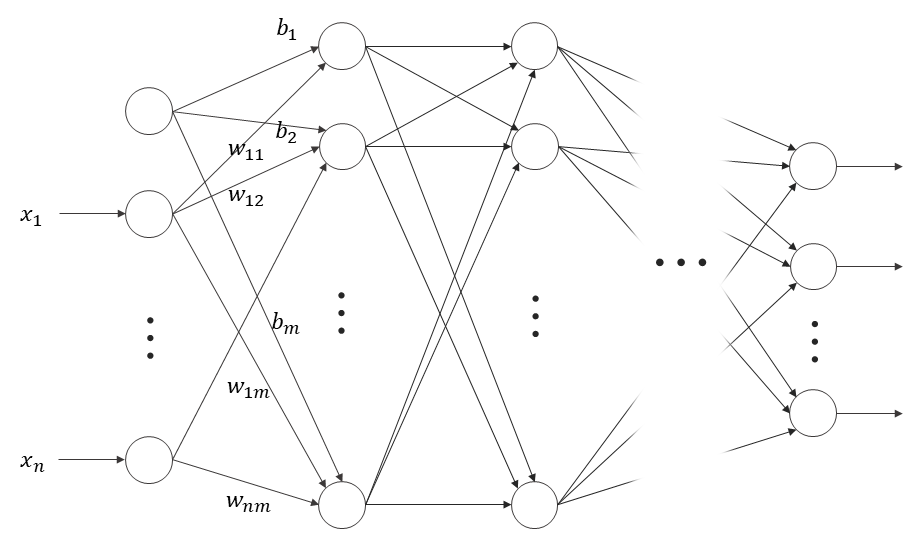
\includegraphics[keepaspectratio, width=120mm]{img/nn.png}
	\caption{ニューラルネットワーク}
	\label{fig_nn}
\end{figure}

\begin{align}
  \bm{h}_{\bm{W},~ \bm{b}}(\bm{X}) &= \bm{\phi}(\bm{X}\bm{W} + \bm{b}) \label{nn_layer}
  \\
  \nonumber
  \\
  \bm{X} &= 
  \begin{bmatrix}
    & x_1 & x_2 & \cdots & x_n  &
  \end{bmatrix}
  \label{nn_x}
  \\
  \nonumber
  \\
  \bm{W} &=
  \begin{bmatrix}
    & w_{11} & w_{12} & \cdots & w_{1m} & \\
    & w_{21} & w_{22} & \cdots & w_{2m} & \\
    & \vdots & \vdots & \ddots & \vdots & \\
    & w_{n1} & w_{n2} & \cdots & w_{nm} & \\
  \end{bmatrix}
  \label{nn_w}
  \\
  \nonumber
  \\
  \bm{b} &=
  \begin{bmatrix}
    & b_1 & b_2 & \cdots & b_n  &
  \end{bmatrix}
  \label{nn_b}
\end{align}

$\bm{X}$は数値化したデータの特徴示す特徴量,
$\bm{W}$はノード間の関係の強さを示す接続重み,
$\bm{b}$は一般に1を要素とするバイアスニューロンと呼ばれるものである.

ニューラルネットワークは脳細胞と似たように,ノード間の関係の強さを調節して機能する.
具体的には,式(\ref{nn_update_weight})に示すように理想の出力$\hat{y}_j$と実際の出力$y_j$の差を利用するなどして次の学習時の接続重みを更新する.

\begin{align}
  w_{i, j}^{(next~ step)} &= w_{i, j} + \eta~ (y_j - \hat{y}_j)~ x_i
  \label{nn_update_weight}
  \\
  \eta &= Const.
  \label{nn_learning_rate}
\end{align}

種々のタスクに特化した機械学習モデルは,このニューラルネットワークの各ノードの接続方法や追加の関数を工夫して作成される.

\subsection{教師あり学習}
教師あり学習は,データにラベルと呼ばれる出力の答えの情報を付与する機械学習である\cite{aurellen20}.
ラベルは人間の関与の基に設定されることが多い.

本研究で行うクラス分類は教師あり学習のひとつである.
クラス分類ではクラスのラベルを基にデータの特徴とクラスの関係を学習し,新規にモデルに入力されたデータがどのクラスに属するかを出力する.
% @see 

\subsection{教師なし学習}
教師なし学習は,データにラベルを付与しない機械学習である\cite{aurellen20}.
人間が関与した答えを用いずにデータの傾向を分析する.

本研究で行うクラスタリングは教師なし学習のひとつである.
クラスタリングでは,データの特徴を基に似たデータ同士をクラスに振り分ける.
データの何を特徴とし,何を基に似たデータと判断するかが重要で,目的によって工夫する必要がある.

\subsection{Attention}
Dzmitryらが2014年に提案したAttentionは,株価や文章といったデータ間に関係がある機械学習を行う際,出力データと関わりが強い入力データに効率よく比重を与えるモジュールである\cite{aurellen20}\cite{bahdanau_neural_2016}.
モデルにAttentionを組み込むことで無駄なデータの学習が減り,モデルが過去に学習した内容を忘却しにくくなる.
これにより,30語以上の長い文章の機械翻訳タスクの精度が大幅に向上する.

図\ref{fig_nn}に機械翻訳モデルに組み込まれたAttention機構を示す.

\begin{figure}[ht]
	\centering
	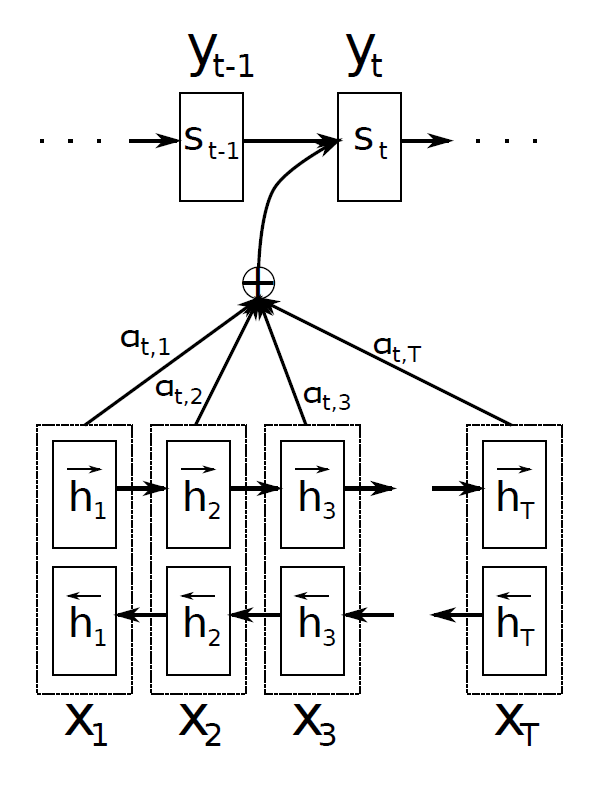
\includegraphics[keepaspectratio, width=120mm]{img/attention.png}
	\caption{入力単語群$(x_1, x_2, ... , x_T)$を基にt番目の出力語$y_t$を生成するAttention機構\cite{bahdanau_neural_2016}}
	\label{attention}
\end{figure}

直前に翻訳した単語$y_{t-1}$と過去に翻訳した単語群の情報$s_{t-1}$に,Attentionの式(\ref{attention_c}))を考慮して次の単語$y_t$を予測している.
$\vec{h_i}$は文脈を加味した単語の意味情報をもつベクトルであり,BiGRUと呼ばれるニューラルネットワークを用いて生成されている.

\begin{align}
  c_{i} &= \sum_{j=1}^{T_{x}} \alpha_{i j} h_{j} &
  \label{attention_c}
  \\
  \alpha_{i j} &= \operatorname*{softmax}_j(e_{ij}) = \frac{\exp \left(e_{i j}\right)}{\sum_{k=1}^{T_{x}} \exp \left(e_{i k}\right)}
  \label{attention_alpha}
  \\
  e_{i j} &= a\left(s_{i-1}, h_{j}\right) = v_{a}^{\top} \tanh \left(W_{a} s_{i-1}+U_{a} h_{j}\right)
  \label{attention_e}
\end{align}

式(\ref{attention_alpha})はソフトマックス関数と呼ばれる関数に式(\ref{attention_e})を代入したものであり$\sum_j \alpha_{ij} = 1$となる意味ベクトル$h_j$の重み係数を表す.
式(\ref{attention_e})は,過去に翻訳した単語群の情報$s_{t-1}$と入力単語の意味ベクトル$h_j$を基に,どの単語に比重を置くかを決定するニューラルネットワークである.
式(\ref{attention_e})の$v_{a}^{\top},~ W_{a},~ U_{a}$はニューラルネットワークの重みである.


\subsection{Transformer(教師なし分類にも触れる)}
~
% @see 

\subsection{BERT}
~
% @see 

\subsection{RoBERTa(BERTとの比較など)}
~
% @see 

%%%%%%%%%%%%%%%%%%%%%%%%%%%%%%
\section{文章分類}
~
% @see 

\subsection{テキストの前処理}
~
% @see 

\subsection{単語埋め込み}
~
% @see 

\subsection{Transformer分類器}
~
% @see 

\subsection{分類モデルの評価(acc, prcなどの議論)}
~
% @see 

%%%%%%%%%%%%%%%%%%%%%%%%%%%%%%
\section{文章の類似度の算出}
~
% @see 

\subsection{Sentence-BERT}
~
% @see 

\subsection{コサイン類似度}
~
% @see 

%%%%%%%%%%%%%%%%%%%%%%%%%%%%%%
\section{クラスタリング}
~
% @see 

\subsection{非階層クラスタリング}
~
% @see 

\subsection{階層的クラスタリング}
~
% @see 

\subsection{Ward法}
~
% @see 

\subsection{(その他使用した手法)}
~
% @see 

\subsection{t-SNE (使うかも)}
~
% @see 


%%%%%%%%%%%%%%%%%%%%%%%%%%%%%%%%%%%%%%%%%%%%%%%%%%%%%%%%%%%%
\chapter{関連研究}
%%%%%%%%%%%%%%%%%%%%%%%%%%%%%%%%%%%%%%%%%%%%%%%%%%%%%%%%%%%%


%%%%%%%%%%%%%%%%%%%%%%%%%%%%%%
\section{ニュース推薦システムのバイアスの解決}
~
% @see 
% [[1]E. BozdagとJ. van den Hoven, 「Breaking the filter bubble: democracy and design」, Ethics Inf Technol, vol. 17, no. 4, pp. 249–265, 12月 2015, doi: 10.1007/s10676-015-9380-y.](https://link.springer.com/article/10.1007/s10676-015-9380-y?source=post_page-----2afbf9cd8367----------------------)
% - フィルターバブルの回避手法
%     - 目標の誤認?
%         - ユーザーに完全なコントロールを付与
%             - バブルの増大も可能に
%                 - (増大せずにコントロールを付与する方法はないか)
%                 - 両方並べて表示すればいいんじゃない
%         - 視点を多様化するよう検索結果を修正
%             - 民主主義の議論に似ている
%             - 完全な民主主義は難しく,本稿では網羅できない

\subsection{Breaking the filter bubble: democracy and design}
~
% @see 

\subsubsection{(UIでバブルの可視化)(結局表示されるものにバイアスがかかる,行動に繋がらない)}
~
% @see 

\subsubsection{(トピックモデル,LSI, LDAの議論)}
~
% @see 

%%%%%%%%%%%%%%%%%%%%%%%%%%%%%%
\section{話題の定量化によるニュース推薦手法}
~
% @see 

\subsection{トピックマップ}
~
% @see 

\subsection{Labeled Bilingual Topic Model for Cross-Lingual Text Classification and Label Recommendation}
~
% @see 

\subsubsection{(LDAの利用)}
~
% @see 

%%%%%%%%%%
% \section{LSI}
~
% @see 

%%%%%%%%%%%%%%%%%%%%%%%%%%%%%%
\section{(要追加調査:比較評価できる推薦手法)(出来事,主張に着目するシステムなど)}
~
% @see 

\subsection{Investigating COVID-19 News Across Four Nations A Topic Modeling and Sentiment Analysis Approach}
~
% @see 

\subsubsection{トピックモデル,top2vec, roberta}
~
% @see 

%%%%%%%%%%
% \section{tf-idf -->}
~%% @see 
 <!-- SCDV -->


%%%%%%%%%%%%%%%%%%%%%%%%%%%%%%%%%%%%%%%%%%%%%%%%%%%%%%%%%%%%
\chapter{提案手法}
%%%%%%%%%%%%%%%%%%%%%%%%%%%%%%%%%%%%%%%%%%%%%%%%%%%%%%%%%%%%


%%%%%%%%%%%%%%%%%%%%%%%%%%%%%%
\section{使用する語彙と基準の定義}
~
% @see 

\subsection{文と文章}
~
% @see 

\subsection{出来事の文}
~
% @see 

\subsection{主張の文}
~
% @see 

\subsection{文が示す話題の類似度}
~
% @see 

%%%%%%%%%%%%%%%%%%%%%%%%%%%%%%
\section{記事の出来事と主張のクラスタを用いた多言語ニュース推薦}
~
% @see 

% フィルターバブル問題を緩和する策として,推薦アルゴリズムの公開,個人が推薦アルゴリズムを管理できるオプションの作成,UIの工夫によるバブルの可視化がある.一方で,個人が推薦アルゴリズムを微調節したところで完全に情報の泡から脱することはできないとの指摘もある.UIでバブル内外を可視化しきるのは不可能 情報が多い 手軽

% (to 提案手法)特定の地域の似た文化と価値観を持つ者同士に向けて記事を提供し,読者にコメントさせる事は,エコーチェンバー問題による情報の偏りを生むと考える.

\subsection{手法概要}
~
% @see 

\subsection{クラスタリングの順序の検討}
~
% @see 

\subsection{(その他報告会などで議論したこと)}
~
% @see 

%%%%%%%%%%%%%%%%%%%%%%%%%%%%%%
\section{データセットの選定}
~
% @see 

\subsection{出来事の文と主張の文の分類器の学習データ(IBM Debater Datasetの議論)}
~
% @see 

\subsection{分類とクラスタリングを行うデータ(covid-19-articlesの議論)}
~
% @see 

%%%%%%%%%%<!-- 
% \section{Japanese fakenews dataset -->}
~
% @see 

%%%%%%%%%%%%%%%%%%%%%%%%%%%%%%
\section{データの前処理}
~
% @see 

\subsection{自然言語処理のためのテキストの前処理(前処理の種類,なぜ前処理するのかなどの議論)}
~
% @see 

\subsection{(その他工夫した前処理)}
~
% @see 


%%%%%%%%%%%%%%%%%%%%%%%%%%%%%%%%%%%%%%%%%%%%%%%%%%%%%%%%%%%%
\chapter{実装}
%%%%%%%%%%%%%%%%%%%%%%%%%%%%%%%%%%%%%%%%%%%%%%%%%%%%%%%%%%%%


%%%%%%%%%%%%%%%%%%%%%%%%%%%%%%
\section{システムの設計指針(入出力,使い方など)}
~
% @see 

%%%%%%%%%%%%%%%%%%%%%%%%%%%%%%
\section{システム構成(モジュールの説明)}
~
% @see 

%%%%%%%%%%%%%%%%%%%%%%%%%%%%%%
\section{実装環境(PCスペック,ライブラリバージョンなど)}
~
% @see 

%%%%%%%%%%%%%%%%%%%%%%%%%%%%%%
\section{データの前処理}
~
% @see 

\subsection{正規表現による前処理(awkの正規表現などの議論)}
~
% @see 

\subsection{省略のピリオドに注意した文章の分割(Stanza, spacyの議論)}
~
% @see 

%%%%%%%%%%%%%%%%%%%%%%%%%%%%%%
\section{出来事の文と主張の文の分類}
~
% @see 

\subsection{Simple Transformers}
~
% @see 

%%%%%%%%%%%%%%%%%%%%%%%%%%%%%%
\section{出来事の文章のクラスタリング}
~
% @see 

\subsection{(要検討)}
~
% @see 

%%%%%%%%%%%%%%%%%%%%%%%%%%%%%%
\section{主張の文のクラスタリング}
~
% @see 

\subsection{(要検討)}
~
% @see 


%%%%%%%%%%%%%%%%%%%%%%%%%%%%%% 
% \section{仮説}
~%% @see 
 評価実験を設計するにあたり以下3件の仮説を立てる.
% \begin{itemize}
%   \item 仮説1) .
%   \item 仮説2) 
%   \item 仮説3) 
% \end{itemize}
% この3件の仮設は,それぞれ以下の考察に基づき設定されている.
% 仮説1は...


%%%%%%%%%%%%%%%%%%%%%%%%%%%%%%%%%%%%%%%%%%%%%%%%%%%%%%%%%%%%
\chapter{実験}
%%%%%%%%%%%%%%%%%%%%%%%%%%%%%%%%%%%%%%%%%%%%%%%%%%%%%%%%%%%%


%%%%%%%%%%%%%%%%%%%%%%%%%%%%%%
\section{出来事の文と主張の文の分類}
~
% @see 

\subsection{実験方法}
~
% @see 

\subsection{実験結果}
~
% @see 

\subsection{実験の考察}
~
% @see 

\subsection{(試行錯誤)}
~
% @see 

%%%%%%%%%%%%%%%%%%%%%%%%%%%%%%
\section{出来事の文章のクラスタリング}
~
% @see 

\subsection{実験方法}
~
% @see 

\subsection{実験結果}
~
% @see 

\subsection{実験の考察}
~
% @see 

\subsection{(試行錯誤)}
~
% @see 

%%%%%%%%%%%%%%%%%%%%%%%%%%%%%%
\section{主張の文のクラスタリング}
~
% @see 

\subsection{実験方法(クラスタの階層の基準ごとの評価)}
~
% @see 

\subsection{実験結果}
~
% @see 

\subsection{実験の考察}
~
% @see 

\subsection{(試行錯誤)}
~
% @see 

%%%%%%%%%%%%%%%%%%%%%%%%%%%%%%
\section{(他の研究との比較実験)}
~
% @see 

\subsection{実験方法}
~
% @see 

\subsection{実験結果}
~
% @see 

\subsection{実験の考察}
~
% @see 

\subsection{(試行錯誤)}
~
% @see 


%%%%%%%%%%%%%%%%%%%%%%%%%%%%%%%%%%%%%%%%%%%%%%%%%%%%%%%%%%%%
\chapter{結果と考察}
%%%%%%%%%%%%%%%%%%%%%%%%%%%%%%%%%%%%%%%%%%%%%%%%%%%%%%%%%%%%


%%%%%%%%%%%%%%%%%%%%%%%%%%%%%%
\section{既存手法との比較}
~
% @see 

%%%%%%%%%%%%%%%%%%%%%%%%%%%%%%
\section{提案手法の妥当性}
~
% @see 

\subsection{入力と出力の妥当性}
~
% @see 

\subsection{処理速度の妥当性(分散システムの議論も)}
~
% @see 

%%%%%%%%%%%%%%%%%%%%%%%%%%%%%%
\section{(結果を基に検討)}
~
% @see 

%%%%%%%%%%%%%%%%%%%%%%%%%%%%%%%%%%%%%%%%%%%%%%%%%%%%%%%%%%%%
\chapter{まとめと展望}
%%%%%%%%%%%%%%%%%%%%%%%%%%%%%%%%%%%%%%%%%%%%%%%%%%%%%%%%%%%%


%%%%%%%%%%%%%%%%%%%%%%%%%%%%%%
\section{まとめ}
~
% @see 

%%%%%%%%%%%%%%%%%%%%%%%%%%%%%%
\section{今後の展望}
~%% @see 
 \section{データセットの相性(ディベートとニュース)}
~
% @see 

%%%%%%%%%%%%%%%%%%%%%%%%%%%%%%%%%%%%%%%%%%%%%%%%%%%%%%%%%%%%
\chapter*{謝辞}
\addcontentsline{toc}{chapter}{謝辞}
%%%%%%%%%%%%%%%%%%%%%%%%%%%%%%%%%%%%%%%%%%%%%%%%%%%%%%%%%%%%

(参考文献は最後に整形します)

%%%%%%%%%%%%%%%%%%%%%%%%%%%%%%%%%%%%%%%%%%%%%%%%%%%%%%%%%%%%
\bibliographystyle{junsrt}
\bibliography{ref.bib}
%%%%%%%%%%%%%%%%%%%%%%%%%%%%%%%%%%%%%%%%%%%%%%%%%%%%%%%%%%%%

\end{document}
